%% Supplementary material for the HarvestMem manuscript (v0.4). Table/figure numbers are referenced from main.tex as S1, S2, ...
\documentclass[preprint,12pt,authoryear]{elsarticle}

\usepackage{lmodern}
\usepackage{amsmath,amssymb}
\usepackage{graphicx}
\usepackage{booktabs}
\usepackage{array}
\usepackage{xcolor}
\usepackage{xr-hyper}
\usepackage[colorlinks=true,linkcolor=blue!50!black,citecolor=blue!50!black,urlcolor=blue!50!black]{hyperref}
\usepackage{adjustbox}
\usepackage[font=small,labelfont=bf,skip=4pt]{caption}
\setlength{\emergencystretch}{2em}

\graphicspath{{../figures/}}
\externaldocument[M-]{main}
\newcommand{\mref}[1]{\ref*{M-#1}}
\newcommand{\tbd}[1]{\textcolor{red}{[TBD: #1]}}
\newcommand{\pekm}{PEKM}
\newcommand{\fdm}{SAM-FDM}
\newcommand{\bench}{HarvestMem-Sim}

\renewcommand{\thesection}{S\arabic{section}}
\renewcommand{\thetable}{S\arabic{table}}
\renewcommand{\thefigure}{S\arabic{figure}}
\renewcommand{\theequation}{S\arabic{equation}}

\journal{Biosystems Engineering}

\begin{document}

\begin{frontmatter}
\title{Supplementary material for ``HarvestMem: event-centric memory for vision--\hspace{0pt}language--\hspace{0pt}action harvesting robots under foliage occlusion''}
\end{frontmatter}

This document contains the material referenced from the main text as Sections~S1--S4, Tables~S1--S3 and Fig.~S1: benchmark details, event detection for every radius, further examples of the frames held by each memory, and the perception-to-memory chain broken down by task. Section, equation, table and figure numbers without the prefix ``S'' refer to the main text.

%% ---------------------------------------------------------------------------
\section{Benchmark details}
\label{sec:s_benchmark}
Each episode of \bench\ samples a tree with a trunk, branches and leaf clusters and 4--6 spherical fruits (radius 2.5--2.9~cm; heights 0.44--0.64~m; distances 0.38--0.50~m from the robot base; azimuth within $\pm 28^\circ$). The layout sampler guarantees that each fruit has a horizontal-approach inverse-kinematics solution, that no branch blocks its approach corridor, and that fruits do not occlude each other in the front camera. A fruit is kinematically attached to its stem until it has been held between both fingers for two consecutive control steps; it then becomes a dynamic rigid body. A demonstrator attempt that fails (planning failure, no detachment, missed basket, task not completed) is discarded and the seed is advanced. Training, validation and test seeds use base seeds 100000, 200000 and 300000. Table~\ref{tab:s_occlusion} quantifies occlusion and the phase structure of the demonstrations.

\begin{table}[h]
\centering
\caption{Occlusion and phase structure (clean training set).}
\label{tab:s_occlusion}
\small
\begin{adjustbox}{max width=\textwidth}\begin{tabular}{lc}
\toprule
Quantity & Value\\
\midrule
Leaf clusters per FruitOccludedRipe episode & 2 (66\% hide a ripe fruit)\\
Occluded fruits fully invisible in the front camera after the gust & 100\%\\
Frames (fruit still on tree) in which an occluded fruit is invisible & mean 72\%, median 78\%\\
Visible fraction of non-occluded fruits after the gust (median) & 1.00\\
Ripe / unripe fruits per FruitOccludedRipe episode & 2.54 / 2.15\\
Mean steps per phase, FruitCount (observe / reach / approach / grasp / & 30 / 118 / 59 / 29 /\\
\quad pull / carry / release / settle) & 58 / 117 / 23 / 34\\
\bottomrule
\end{tabular}\end{adjustbox}
\end{table}

%% ---------------------------------------------------------------------------
\section{Event detection versus radius}
\label{sec:s_events}
Table~\ref{tab:s_radius} gives event detection from the ground-truth distance for every radius evaluated (plotted in Fig.~\mref{fig:events}a of the main text). The radius used throughout ($r=3$~cm) was selected on the training set; the plateau of exact detection between 1 and 4~cm is bounded below by how close the gripper comes to the fruit centre and above by half the inter-fruit spacing. The robustness of detection to perturbations of the distance signal is reported in Table~\mref{tab:robust} of the main text.

\begin{table}[h]
\centering
\caption{Event detection versus radius $r$ (tol = 5 mm, ground-truth distance). Train: 200 episodes; validation: 199 episodes with 2--5 picks each. Count: fraction of validation episodes with the exact pick count.}
\label{tab:s_radius}
\small
\begin{adjustbox}{max width=\textwidth}\begin{tabular}{lcccccccc}
\toprule
 & \multicolumn{3}{c}{Training} & \multicolumn{3}{c}{Validation} & \\
\cmidrule(lr){2-4}\cmidrule(lr){5-7}
$r$ (cm) & P & R & F1 & P & R & F1 & Count\\
\midrule
0.5 & 0.982 & 0.603 & 0.747 & 0.968 & 0.628 & 0.762 & 0.30\\
1 & 1.000 & 1.000 & 1.000 & 1.000 & 1.000 & 1.000 & 1.00\\
2 & 1.000 & 1.000 & 1.000 & 1.000 & 1.000 & 1.000 & 1.00\\
\textbf{3 (used)} & \textbf{1.000} & \textbf{1.000} & \textbf{1.000} & \textbf{1.000} & \textbf{1.000} & \textbf{1.000} & \textbf{1.00}\\
4 & 1.000 & 1.000 & 1.000 & 1.000 & 1.000 & 1.000 & 1.00\\
5 & 0.996 & 1.000 & 0.998 & 0.998 & 1.000 & 0.999 & 0.99\\
6 & 0.971 & 1.000 & 0.985 & 0.962 & 1.000 & 0.981 & 0.91\\
8 & 0.788 & 1.000 & 0.881 & 0.813 & 1.000 & 0.897 & 0.67\\
10 & 0.647 & 1.000 & 0.786 & 0.692 & 1.000 & 0.818 & 0.49\\
\bottomrule
\end{tabular}\end{adjustbox}
\end{table}



%% ---------------------------------------------------------------------------
\section{Further examples of memory content}
\label{sec:s_timelines}
Figure~\ref{fig:s_timelines} extends Fig.~\mref{fig:timeline} of the main text to three further validation episodes, taken in order from the first episodes of each task and chosen to show the three regimes predicted by the coverage analysis rather than favourable cases. In a long FruitCount episode with five picks (a), uniform memory covers none of the picks at the last decision, \pekm\ with $k=4$ the two most recent and with $k=8$ the four most recent (its cap), and PEKM-S four of five but not the most recent one, the weakness of the soft variant noted in Section~\mref{sec:res_memory}. In a FruitOccludedRipe episode with three picks (b), uniform memory keeps only the first. In a short episode with two picks (c), the uniform grid is dense enough to cover both, as Eq.~(\mref{eq:coverage}) predicts for small $t$, and all memories agree.

\begin{figure}[h]
\centering
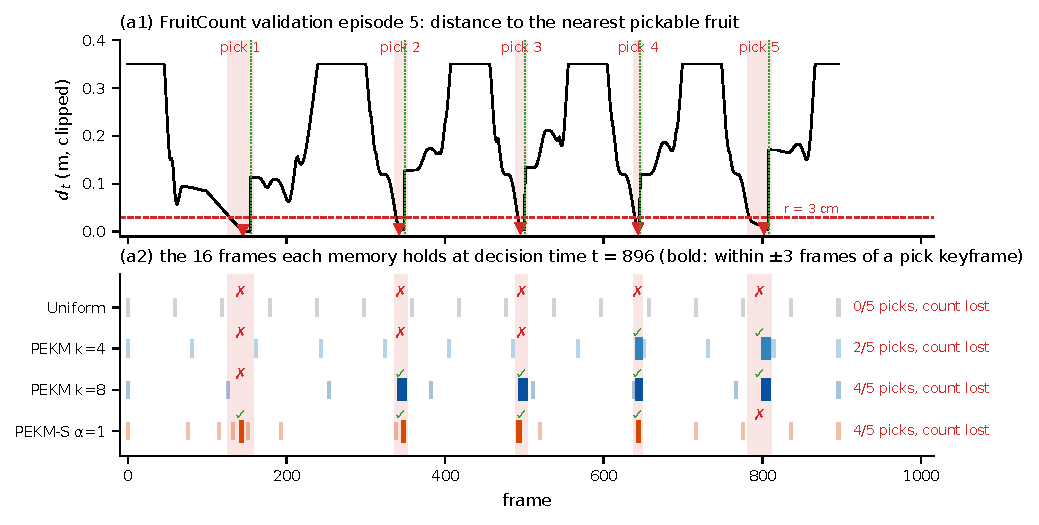
\includegraphics[width=\linewidth]{figS_timeline_a}\\[4pt]
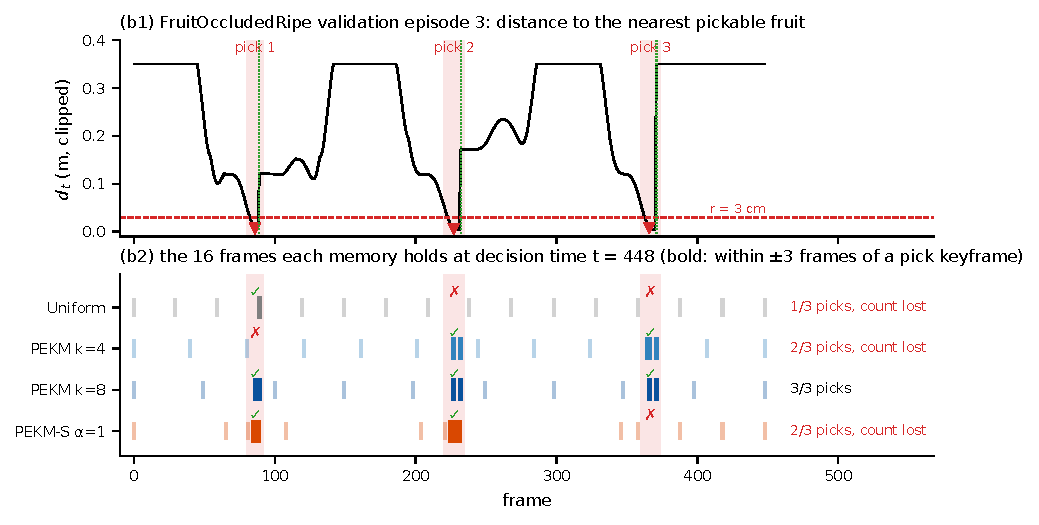
\includegraphics[width=\linewidth]{figS_timeline_b}\\[4pt]
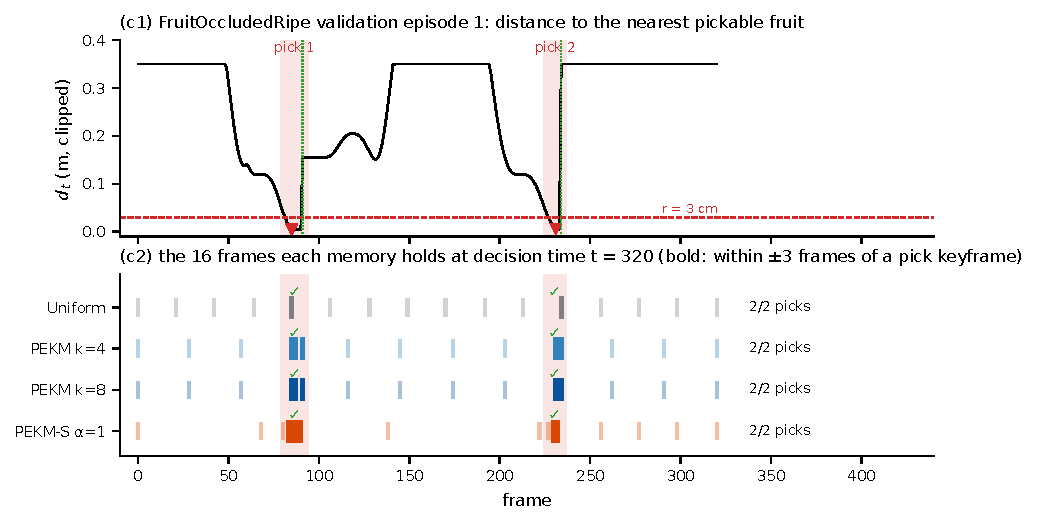
\includegraphics[width=\linewidth]{figS_timeline_c}
\caption{Frames held by 16-frame memories in three further validation episodes: (a) FruitCount episode 5 (five picks, $t=896$), (b) FruitOccludedRipe episode 3 (three picks, $t=448$), (c) FruitOccludedRipe episode 1 (two picks, $t=320$). Layout as in Fig.~\mref{fig:timeline} of the main text: top, the TCP-to-fruit distance with detected picks and their $\pm3$-frame key windows (shaded), contact keyframes (triangles), the radius (dashed) and detachments (dotted); bottom, the frames held at the last decision, bold within $\pm3$ frames of a pick keyframe, with \textcolor{green!50!black}{\checkmark}\,/\,\textcolor{red}{$\times$} marking whether each pick is covered.}
\label{fig:s_timelines}
\end{figure}

%% ---------------------------------------------------------------------------
\section{Perception-to-memory chain by task}
\label{sec:s_chain}
Table~\ref{tab:s_chain} breaks down Table~\mref{tab:chain} of the main text by task and adds the K8 memory. Two task-specific effects stand out. First, post-gust anchors affect only FruitOccludedRipe, where they lose every leaf-hidden ripe fruit (Section~\mref{sec:res_anchor} of the main text), while in FruitCount they coincide with frame-0 anchors. Second, per-frame detection without anchors produces more spurious events in FruitCount (precision 0.759, count exact 0.46) than in FruitOccludedRipe (0.906, 0.77). Its failure mode, the carried fruit being detected as the nearest fruit, occurs once per carrying phase, and FruitCount episodes contain more picks (2.9 versus 2.5 on average). The delay of depth-only vacancy is the same in both tasks (median 16 frames), as expected from its cause, the arm and the carried fruit hiding the vacated anchor while carrying.

\begin{table}[h]
\centering
\caption{Events and memory from perceived distances, by task (plain detector; hysteresis in parentheses where it differs). Dist.\ err.: median / 90th-percentile error of $\hat d_t$ where $d_t \le 10$ cm (--: no fruit perceived in more than 10\% of near-range frames). Rel.\ err.: median release-keyframe error (frames). J4, J8: Jaccard similarity of the K4 and K8 memories to the ground-truth memory; KF4, KF8: recall of ground-truth keyframes within $\pm3$ frames.}
\label{tab:s_chain}
\footnotesize
\setlength{\tabcolsep}{3.5pt}
\begin{adjustbox}{max width=\textwidth}\begin{tabular}{lcccccccccc}
\toprule
Distance source & Dist.\ err.\ (cm) & P & R & F1 & Count & Rel.\ err. & J4 & J8 & KF4 & KF8\\
\midrule
\multicolumn{11}{l}{\emph{FruitCount} (99 episodes, 287 picks)}\\
GT (upper bound) & 0 / 0 & 1.000 & 1.000 & 1.000 & 1.00 & 0 & 1.000 & 1.000 & 1.000 & 1.000\\
\fdm\ (ours) & 0.33 / 0.48 & 1.000 & 1.000 & 1.000 & 1.00 & 0 & 0.947 & 0.937 & 1.000 & 1.000\\
\fdm\ + depth noise & 0.30 / 0.45 & 1.000 & 1.000 & 1.000 & 1.00 & 0 & 0.948 & 0.939 & 1.000 & 1.000\\
Depth-only & 0.41 / 11.24 & 1.000 & 1.000 & 1.000 & 1.00 & 16 & 0.684 & 0.651 & 0.842 & 0.842\\
Post-gust anchors & 0.33 / 0.48 & 1.000 & 1.000 & 1.000 & 1.00 & 0 & 0.947 & 0.937 & 1.000 & 1.000\\
Per-frame & 0.42 / 12.95 & 0.759 (0.920) & 1.000 & 0.863 (0.958) & 0.46 (0.79) & 52 & 0.437 & 0.366 & 0.740 & 0.775\\
\midrule
\multicolumn{11}{l}{\emph{FruitOccludedRipe} (100 episodes, 251 picks)}\\
GT (upper bound) & 0 / 0 & 1.000 & 1.000 & 1.000 & 1.00 & 0 & 1.000 & 1.000 & 1.000 & 1.000\\
\fdm\ (ours) & 0.35 / 0.48 & 1.000 & 1.000 & 1.000 & 1.00 & 0 & 0.948 & 0.944 & 1.000 & 1.000\\
\fdm\ + depth noise & 0.32 / 0.47 & 1.000 & 1.000 & 1.000 & 1.00 & 0 & 0.948 & 0.944 & 1.000 & 1.000\\
Depth-only & 0.38 / 7.81 & 1.000 & 1.000 & 1.000 & 1.00 & 16 & 0.687 & 0.671 & 0.849 & 0.855\\
Post-gust anchors & 5.78 / -- & 1.000 & 0.450 & 0.621 & 0.00 & 0 & 0.493 & 0.479 & 0.731 & 0.734\\
Per-frame & 0.36 / 11.91 & 0.906 (0.969) & 1.000 & 0.951 (0.984) & 0.77 (0.92) & 52 & 0.402 & 0.360 & 0.773 & 0.790\\
\bottomrule
\end{tabular}\end{adjustbox}
\end{table}


\end{document}
